\documentclass[12pt]{article}
\usepackage{amsmath, amssymb, amsthm, graphicx, epsfig, fancyhdr, graphicx, amsfonts}
\usepackage{algorithm}
\usepackage[noend]{algpseudocode}
\usepackage[utf8]{inputenc}

\title{Math 240 Overleaf Form} 
\author {Laouen belloli}

\setlength{\headheight}{28pt}
\pagestyle{fancy}
\fancyhf{}
\fancyhead[R]{Laouen Belloli \\ Automatic creation of Metabolic Network in PDEVS}
\fancyfoot[C]{\thepage}


\begin{document}

\section*{summary of the reading}
After spend 3 days reading both books,''Principles of Biochimistry`` from Lehninger and ''Chemistry \& Chemical Reactions``  from Kotz \& Treichel, I restart with another diferent aprouch to the problem.

Since we only want to consider reaction leaded by enzymes, I don't see why to model the reactions instead of model the cell components. A cell have many components and fenomens, but we can only model these components and fenomen that we need. In this way, in the future, we can add others components or fenomens as we'll need it.


\section*{new aprouch for the cell model}  
A cell have basicly three components, a wall (membrane) a cytoplasm (where some reaction happens) and organelles (diferents compartments with theirs reactions).
There is a lot of other components but I am not considering them.
Both, the citoplasm and the organelles have enzymes and therefore reaction happens there. also both have walls. The main diference is that the organelles are conected only with the cytoplasm while the cytoplasm is conected with all the organelles and to the cell wall.

my Idea now is to model the next components: the enzymes, the organelles, the cytoplasm and the space like a discrete tridimensional space in $\mathbb{Z}^3$. The molecules now can be the input and output, and their are only in the messages and models states.

\newpage
\subsection*{the Filter model}
Since BCDPP (Boost CD++) has no ports, all models have a filter to ignore the messages that are not directed to the them.
The next FSM explain the behavior of a atomic Filter model.


\begin{figure}[h!]
 \centering
  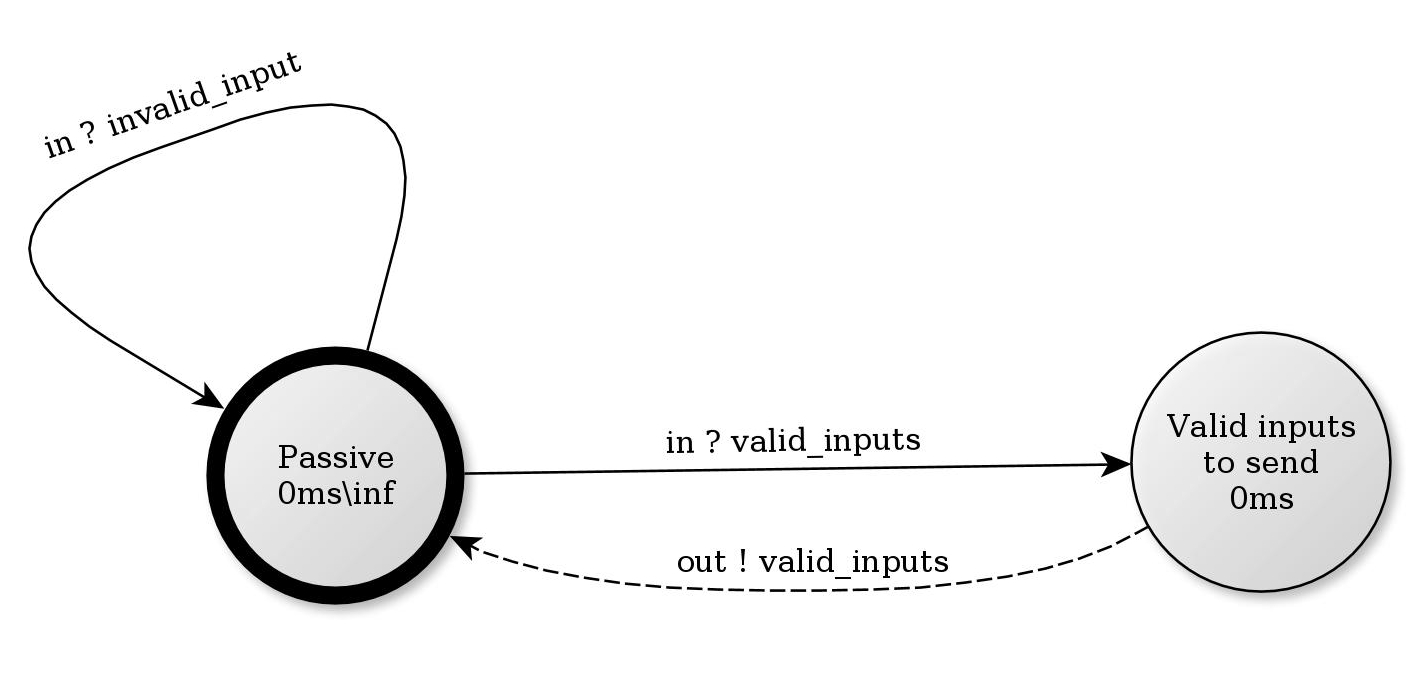
\includegraphics[width=1\textwidth]{atomic-filter.jpg}
 \caption{Atomic Filter model.}
\end{figure}

\newpage
\subsection*{the enzyme}
The coupled model for a enzyme is the next:

\begin{figure}[h!]
 \centering
  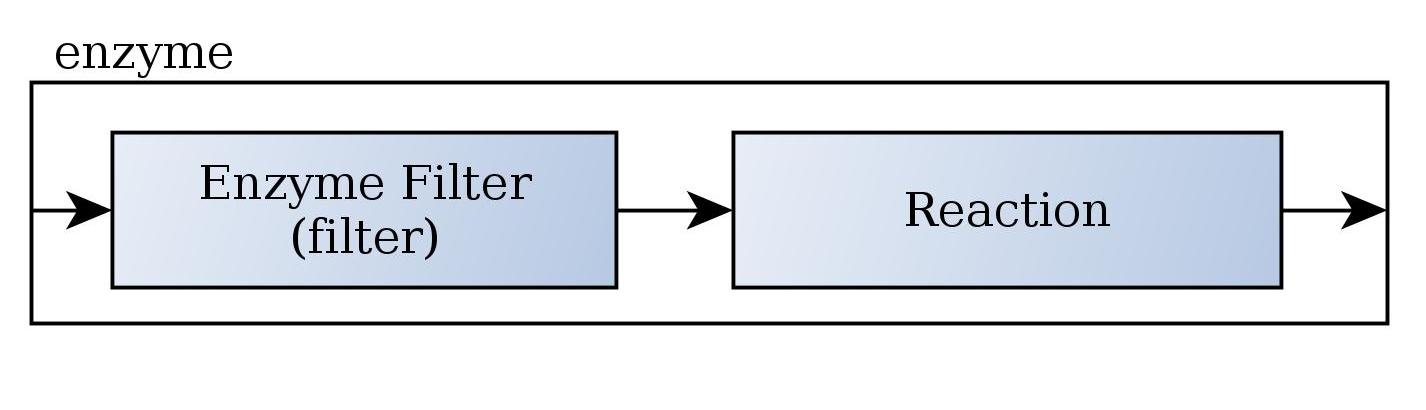
\includegraphics[width=1\textwidth]{coupled-enzyme.jpg}
 \caption{enzyme coupled model.}
\end{figure}


The next FSM model introduce the behavior of the atomic Reaction model.

\begin{figure}[h!]
 \centering
  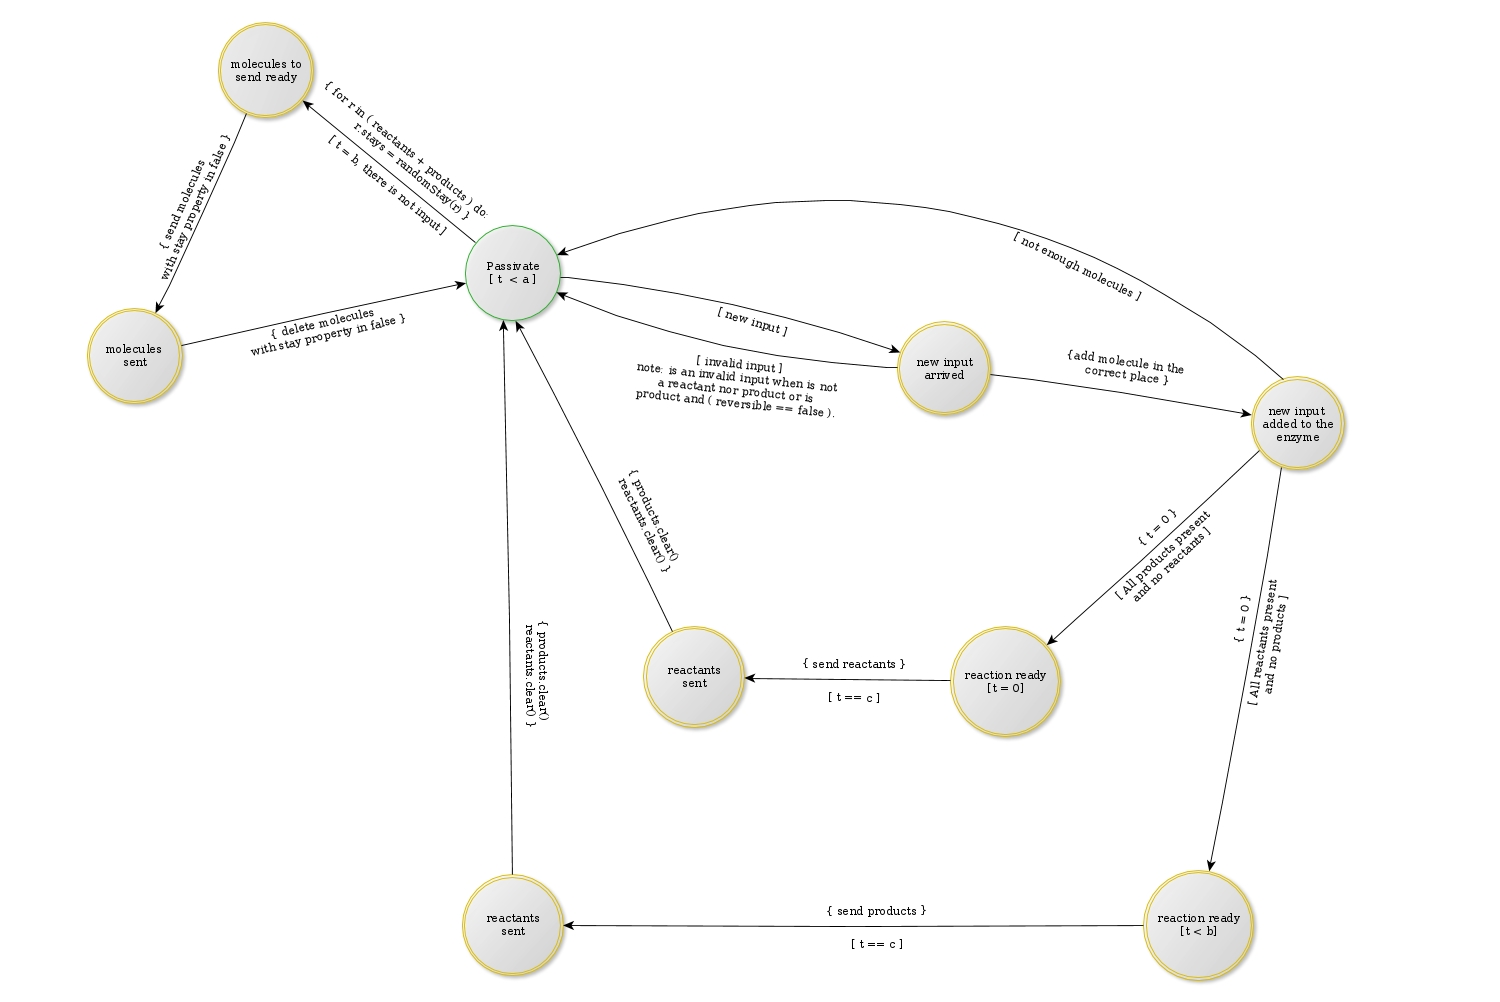
\includegraphics[width=1\textwidth]{atomic-enzyme.jpg}
 \caption{Atomic Reaction model.}
\end{figure}

When an input arrive to the enzyme is attached to the enzyme for a random time if all the necesary elements are in the enzyme in the same time, the reaction will start taken a determinated rate time to finish and send the output and clear the enzyme to restart the proces.
every constant time interval, the enzyme look if one of the current attached element will be dettached with a random function.



\end{document}